\documentclass[a4paper,11pt,leqno]{article}
%-------------------------------------------------------------------------------
\usepackage[czech]{babel}
\usepackage[utf8]{inputenc}
\usepackage[left=2cm,top=3cm,text={17cm,24cm}]{geometry}
\usepackage[usenames, dvipsnames]{color}
\usepackage{graphicx}
\usepackage{pdflscape}
%-------------------------------------------------------------------------------
\definecolor{green1}{RGB}{0, 120, 0}
\definecolor{red1}{RGB}{196, 0, 0}
\definecolor{yellow1}{RGB}{229, 229, 0}
%-------------------------------------------------------------------------------
\begin{document}
%-------------------------------------------------------------------------------
%-----------
% Title PAGE
%-----------
\begin{titlepage}
	\begin{center}
		{\Huge                
		\textsc{Vysoké učení technické v~Brně}}		\\[1em]
		{\huge
		\textsc{Fakulta informačních technologií}}  \\

		\begin{figure}[h]
			\begin{center}
				\scalebox{0.75}{
\includegraphics{images/fit-logo.eps}}
			\end{center}
		\end{figure}
	
		\vspace{\stretch{0.382}}
		{\LARGE
		Dokumentace k~projektu do IFJ/IAL}	\\[3ex]
		{\Huge\textbf{Implementace překladače imperativního jazyka IFJ17}}	\\[1.5ex]
		{\Huge Tým 022, varianta II}	\\
		\vspace{\stretch{0.618}}
	\end{center}
		{\Large
	\textbf{Členové týmu}:	\\
		\begin{tabular}{lclc}
Martin Omacht  	& -- & xomach00 (vedoucí) 	& 34\,\%	\\
Zdeněk Chovanec & -- & xchova19				& 33\,\%	\\
Petr Hendrych 	& -- & xhendr03 			& 33\,\%
		\end{tabular}} \\[3ex]
		{\Large \textbf{Rozšíření}: BASE, UNARY, FUNEXP, BOOLOP, IFTHEN, CYCLES} \\[3ex]
		\begin{flushright}
			{\Large 6. prosince 2017}
		\end{flushright}
\end{titlepage}
%-------------------------------------------------------------------------------
%-----
% TEXT
%-----
\section{Úvod}
Cílem projektu bylo vytvoření překladače pro imperativní jazyk IFJ17.
Jazyk IFJ17 je podmnožinou jazyka FreeBASIC, který je založen na jazyce BASIC.
Při registracích jsme si vybrali variantu II, která spočívala v řešení projektu za pomoci tabulky s~rozptýlenými položkami.
Následuje výčet etap, tak jak šly za sebou.
%-------------------------------------------------------------------------------
\section{Etapy projektu}
Projekt jsme zahájili vytvořením prostředí pro vývoj.
To zahrnovalo prvotní nastavení využitých nástrojů.
Jelikož se preference operačních systemů mezi členy týmu liší, jako sestavovací
program jsme zvolili nástroj \textbf{CMake}. Pro účely testování byl využit
framework \textbf{Googletest}.
%-------------------------------------------------------------------------------
\subsection{Lexikální analyzátor (LA)}
Návrh LA byl prvním krokem k~vytvoření překladače.
Při návrhu deterministického konečného automatu, na kterém je LA založen jsme se snažili striktně dodržovat specifikaci jazyka IFJ17.
Samotná implementace koresponduje s~tímto schematickým návrhem (viz obrázek \ref{pic_scanner}, strana \pageref{pic_scanner}) téměř jednu ku jedné.
Lexikální analyzátor je samostatná jednotka, jejíž činnost je plně podřízena syntaktickému analyzátoru.
V~počátečních fázích vývoje byla komunikace mezi syntaktickým a lexikálním analyzátorem
jednosměrná -- SA v~případě potřeby zavolal LA, který ze vstupu načetl další token.
V~průběhu vývoje jsme ale dospěli k~závěru, že bude výhodnější umožnit komunikaci oběma směry.
Komunikace ve směru SA $\rightarrow$ LA se projevuje tak, že SA má možnost vrátit LA právě načtený token.
V~prípadě, že SA v~tuto chvíli zažádá o~další token, LA nebude načítat \uv{nový} token ze vstupu, nýbrž mu poskytne \uv{starý} token, který mu byl vrácen samotným SA.
\subsection{Syntaktický analyzátor (SA)}
\subsubsection{Analýza konstrukcí a příkazů (bez výrazů)}
Pro vyhodnocení této části programů jsme se rozhodli použit metodu prediktivní syntaktické analýzy řízené LL tabulkou.
Důvod, proč jsme nezvolili doporučenou metodu je ten, že prediktivní analýza se nám jevila jako efektivnější a sofistikovanější řešení.
Největší výzvou této etapy byl návrh LL gramatiky. Následné sestavení LL tabulky, pomocí postupů, které nám byly prezentovány na přednáškách, již nepředstavovalo větší problém.
Jak LL gramatika, tak i LL tabulka jsou součástí překladače a jsou inicializovány při spuštění programu.
LL gramatika je implementována jako pole pravidel, kde prvku na indexu \emph{n} odpovidá pravidlo číslo \emph{n} v~návrhu gramatiky (strana \pageref{ll_grammar}).
Jelikož je velká část LL tabulky prázdná, rozhodli jsme se ji implementovat jako řidkou tabulku.
\subsubsection{Analýza výrazů}
Analýza výrazů je prováděna za pomoci precedenční tabulky a přidružených gramatických pravidel.
Již od počátku jsme zamýšleli implementovat rozšíření FUNEXP a UNARY,
která se podepsala na výsledné podobě precedenční tabulky.
%-------------------------------------------------------------------------------
\subsection{Sémantická analýza}
Tato část pro náš tým představovala největší výzvu.
Problém jsme vyřešili následujícím způsobem. Vybraným pravidlům LL gramatiky jsme
přiřadili příznak sémantické akce (zkratka: sém. akce).
Každá sém. akce reprezentuje stavový automat, který při zpracování jednoho vstupu může přejít do nového stavu, nebo zůstat ve stavu, ve kterém se aktuálně nachází.
V~případě, že v~průběhu syntaktické analýzy je
na vrcholu syntaktického zásobníku detekován neterminál s~příznakem sém. akce,
je příslušná akce vložena na zásobník sémantických akcí.
Před načtením nové lexémy je zavolána sém. akce z~vrcholu zásobníku a je jí předán
aktuální token. Tato akce má za úkol daný token zpracovat
(například zkontrolovat typ, existenci proměnné, vygenerovat instrukce).
Jestliže akce v~průběhu zpracovávání
svého vstupu dosáhne koncového stavu je odebrána ze zásobníku.
Jelikož na zásobníku může být sém.
akcí hned několik, avšak aktivní je v~daném okamžiku jen ta na vrcholu,
je nutné, aby si sém. akce mezi sebou předávaly informace.
K~předávání informací dochází právě v~okamžiku odstraňování akce ze
zásobníku, kdy je právě dokončená sém. akce odebrána a její výsledek je předán akci, která se nově nachází na vrcholu zásobníku.
\subsubsection{Implementace TS}
Tabulka symbolů je reprezentována tabulkou s~rozptýlenými položkami s~explicitně
zřetězenými synonymy. Synonyma jsou svázána do jednosměrného seznamu a nejsou
seřazena. V případě vkládání položky je daná položka vložena na konec seznamu. Jako mapovací funkci jsme použili funkci DJB.
%-------------------------------------------------------------------------------
\subsection{Generování kódu}
Původní plán byl generovat abstraktní syntaktický strom a následně z~něj
vygenerovat kód, avšak neshledali jsme v tomto řešení žádnou výhodu, ale spíše jen
časové zdržení. Proto jsme se rozhodli generovat instrukce tří adresného kódu přímo.
Instrukce jsou generovány do tří různých seznamů.
\begin{enumerate}
	\item{\textbf{globální seznam} -- definice globálních proměnných a jejich inicializace}
	\item{\textbf{seznam pro funkce} -- definice funkcí}
	\item{\textbf{instrukce hlavního těla programu}}
\end{enumerate}
Na konci analýzy celého vstupního programu se nejdříve vypíší instrukce z~globálního seznamu, poté hlavní tělo programu a nakonec funkce.
%-------------------------------------------------------------------------------
\section{Rozdělení práce}
Martin Omacht
\begin{itemize}
	\item{implementace syntaktické analýzy (bez výrazů)}
	\item{implementace sémantické analýzy}
	\item{generování kódu}
	\item{testování}
\end{itemize}
Zdeněk Chovanec
\begin{itemize}
	\item{návrh konečného automatu lexikálního analyzátoru}
	\item{návrh gramatik pro syntaktický analyzátor}
	\item{implementace syntaktické analýzy pro výrazy}
	\item{implementace tabulky symbolů}
\end{itemize}
Petr Hendrych
\begin{itemize}
	\item{implementace lexikálního analyzátoru}
	\item{vestavěné funkce v IFJcode17}
	\item{dokumentace}
	\item{prezentace}
\end{itemize}
%-------------------------------------------------------------------------------
\section{Rozšíření}
\subsection{GLOBAL}
Toto rozšíření přidává možnost definování globálních a statických proměnných.
Implementace globálních proměnných nepředstavovala žádný problém -- jejich definice je
přidána na globální instrukční list a prostor pro ně je alokován na globálním rámci.
Jelikož statické proměnné si musí uchovávat hodnotu mezi jednotlivými volání funkce, bylo to s~nimi složítější.
Vyřešili jsme to tak, že jsme tyto proměnné definovali jako globální.
Zároveň byl k~jejich názvu přidán prefix \uv{S\emph{name}},
kde \emph{name} je název funkce, ve kterých jsou definovány. Tímto nedojde ke
kolizím s~ostatními proměnnými.
\subsection{UNARY}
Implementace operace přiřazení s~aritmetickou operací se jednoduše vyřešilo
provedením aritmetické operace a následným přirazení do proměnné.
U~unárního mínus bylo potřeba přidat jeden sloupec/řádek reprezentující
unární mínus do precedenční tabulky. Problémem však je, že jeden symbol
může značit 2 různé operace. Tento problém jsme vyřešili tak, že v~případě,
že je načten token značící operaci odčítání, je na základě předchozího
načteného tokenu rozhodnuto zda-li se jedná o~minus binární, čí unární.
\subsection{BASE}
Rozšíření ovlivnilo pouze lexikální analyzátor, kde po načtení čísla v~jiné soustavě se převedlo do dekadické soustavy a dále se pracovalo pouze s~dekadickým číslem.
\subsection{CYCLES}
Zde byl nutný zásah do LL gramatiky (resp. LL tabulky). S~tímto 
rozšířením jsme počítali již od začátku, tudíž to nepředstavovalo žádný problém.
Stejně tak doplnění plné funkcionality cyklu typu \textbf{Do\dots Loop}. Největší záludnost se skrývala v~cyklu \textbf{For\dots Next}, a to v~definici iterační proměnné. 
Řešení spočíva v~tom, že každý cyklus \textbf{for} je označen unikátním identifikátorem. V~prípadě, že dojde k~definici nové iterační proměnné, je tato proměnná definována na globálním
rámci a je její jméno tvoří řetězec, který vznikne zkonkatenováním původní názvu
iterační proměnné a identifikátoru cyklu \textbf{for}. Po skončení cyklu již k~této
proměnné nelze přistoupit. Pro implementaci příkazů \textbf{exit}, \textbf{continue} jsme 
použili dříve zmíněný zásobník sémantických akcí.
\subsection{FUNEXP}
Toto rozšíření se implementovalo jednoduše pomoci vyhodnocování výrazů na datovém zásobníku.
Parametry funkcí totiž předáváme datovým zásobníkem, stejně tak i návratovou hodnotu funkce.
Menší problém představovala implicitní konverze datového typu předávaných parametrů při volání funkce.
Parametry již byly vloženy na datový zásobník a nebyl k~nim přístup pro konverzi.
Toto bylo vyřešeno v~definici funkce, kde pokud byl parametr typu INT nebo DOUBLE bylo k nim vygenerováno dynamické přetypování. To spočívalo, v zjištění datového typu pomocí instrukce TYPE a následně přeskočení konverze, pokud datový typ odpovídal definici parametru.
\subsection{IFTHEN}
Podpora IF bez větve ELSE nebyla složitá. U~větví ELSEIF bylo potřeba zajistit podporu pro jejich potenciálně nekonečné množství. Toho bylo docíleno tím, že se pro každou tuto větev vygeneruje unikátní identifikátor.
\subsection{BOOLOP}
V~zásadě se jednalo pouze o~rozšíření precedenční tabulky o~logické operátory.
%-------------------------------------------------------------------------------
\section{Komunikace v~týmu}
Pro online komunikaci jsme si vybrali Messenger, kde jsme si založili skupinový chat. Pokud se však objevil větší problém, tak jsme se sešli všichni osobně.
Pro sdílení souborů projektu a verzování jsme zvolili verzovací systém Git hostovaný na službě Github. Github nám umožňoval například code review nově nahraných verzí nebo přidávání issues pokud něco nefungovalo.
%-------------------------------------------------------------------------------
\section{Projekt v číslech}
\begin{itemize}
	\item{počet řádků: 8 883}
	\item{počet commitů: 342}
	\item{počet souborů: 37}
\end{itemize}
%-------------------------------------------------------------------------------
\section{Shrnutí}
Projekt byl něco zcela nového pro všechny z~nás a zabral opravdu velkou část semestru.
Museli jsme se naučit mnohému jako například: práce v~týmu a komunikace v~něm,
práce s~verzovacím systémem Git, nemluvě o~nabytých znalostech z~oblasti teorie
formálních jazyků. Využili jsme pokusného odevzdání a myslíme, že splnilo
svůj účel. V~těch pár dnech, které mu předcházely, nás totiž přinutilo pracovat
usilovněji, než bychom pracovali za normálních okolností. Samotně vyhodnocení pokusného odevzdání
a relativně dobrý výsledek už byl jen třešníčkou na dortu. Pro nás to znamenalo 
především to, že jsme mohli začít dolaďovat menší nedostatky a implementovat
zbývající rozšíření, na která jsme ještě měli zálusk.
%------------
% Scanner FSM
%------------
\begin{landscape}
\begin{figure}[ht]
	\begin{center}
		\scalebox{0.50}{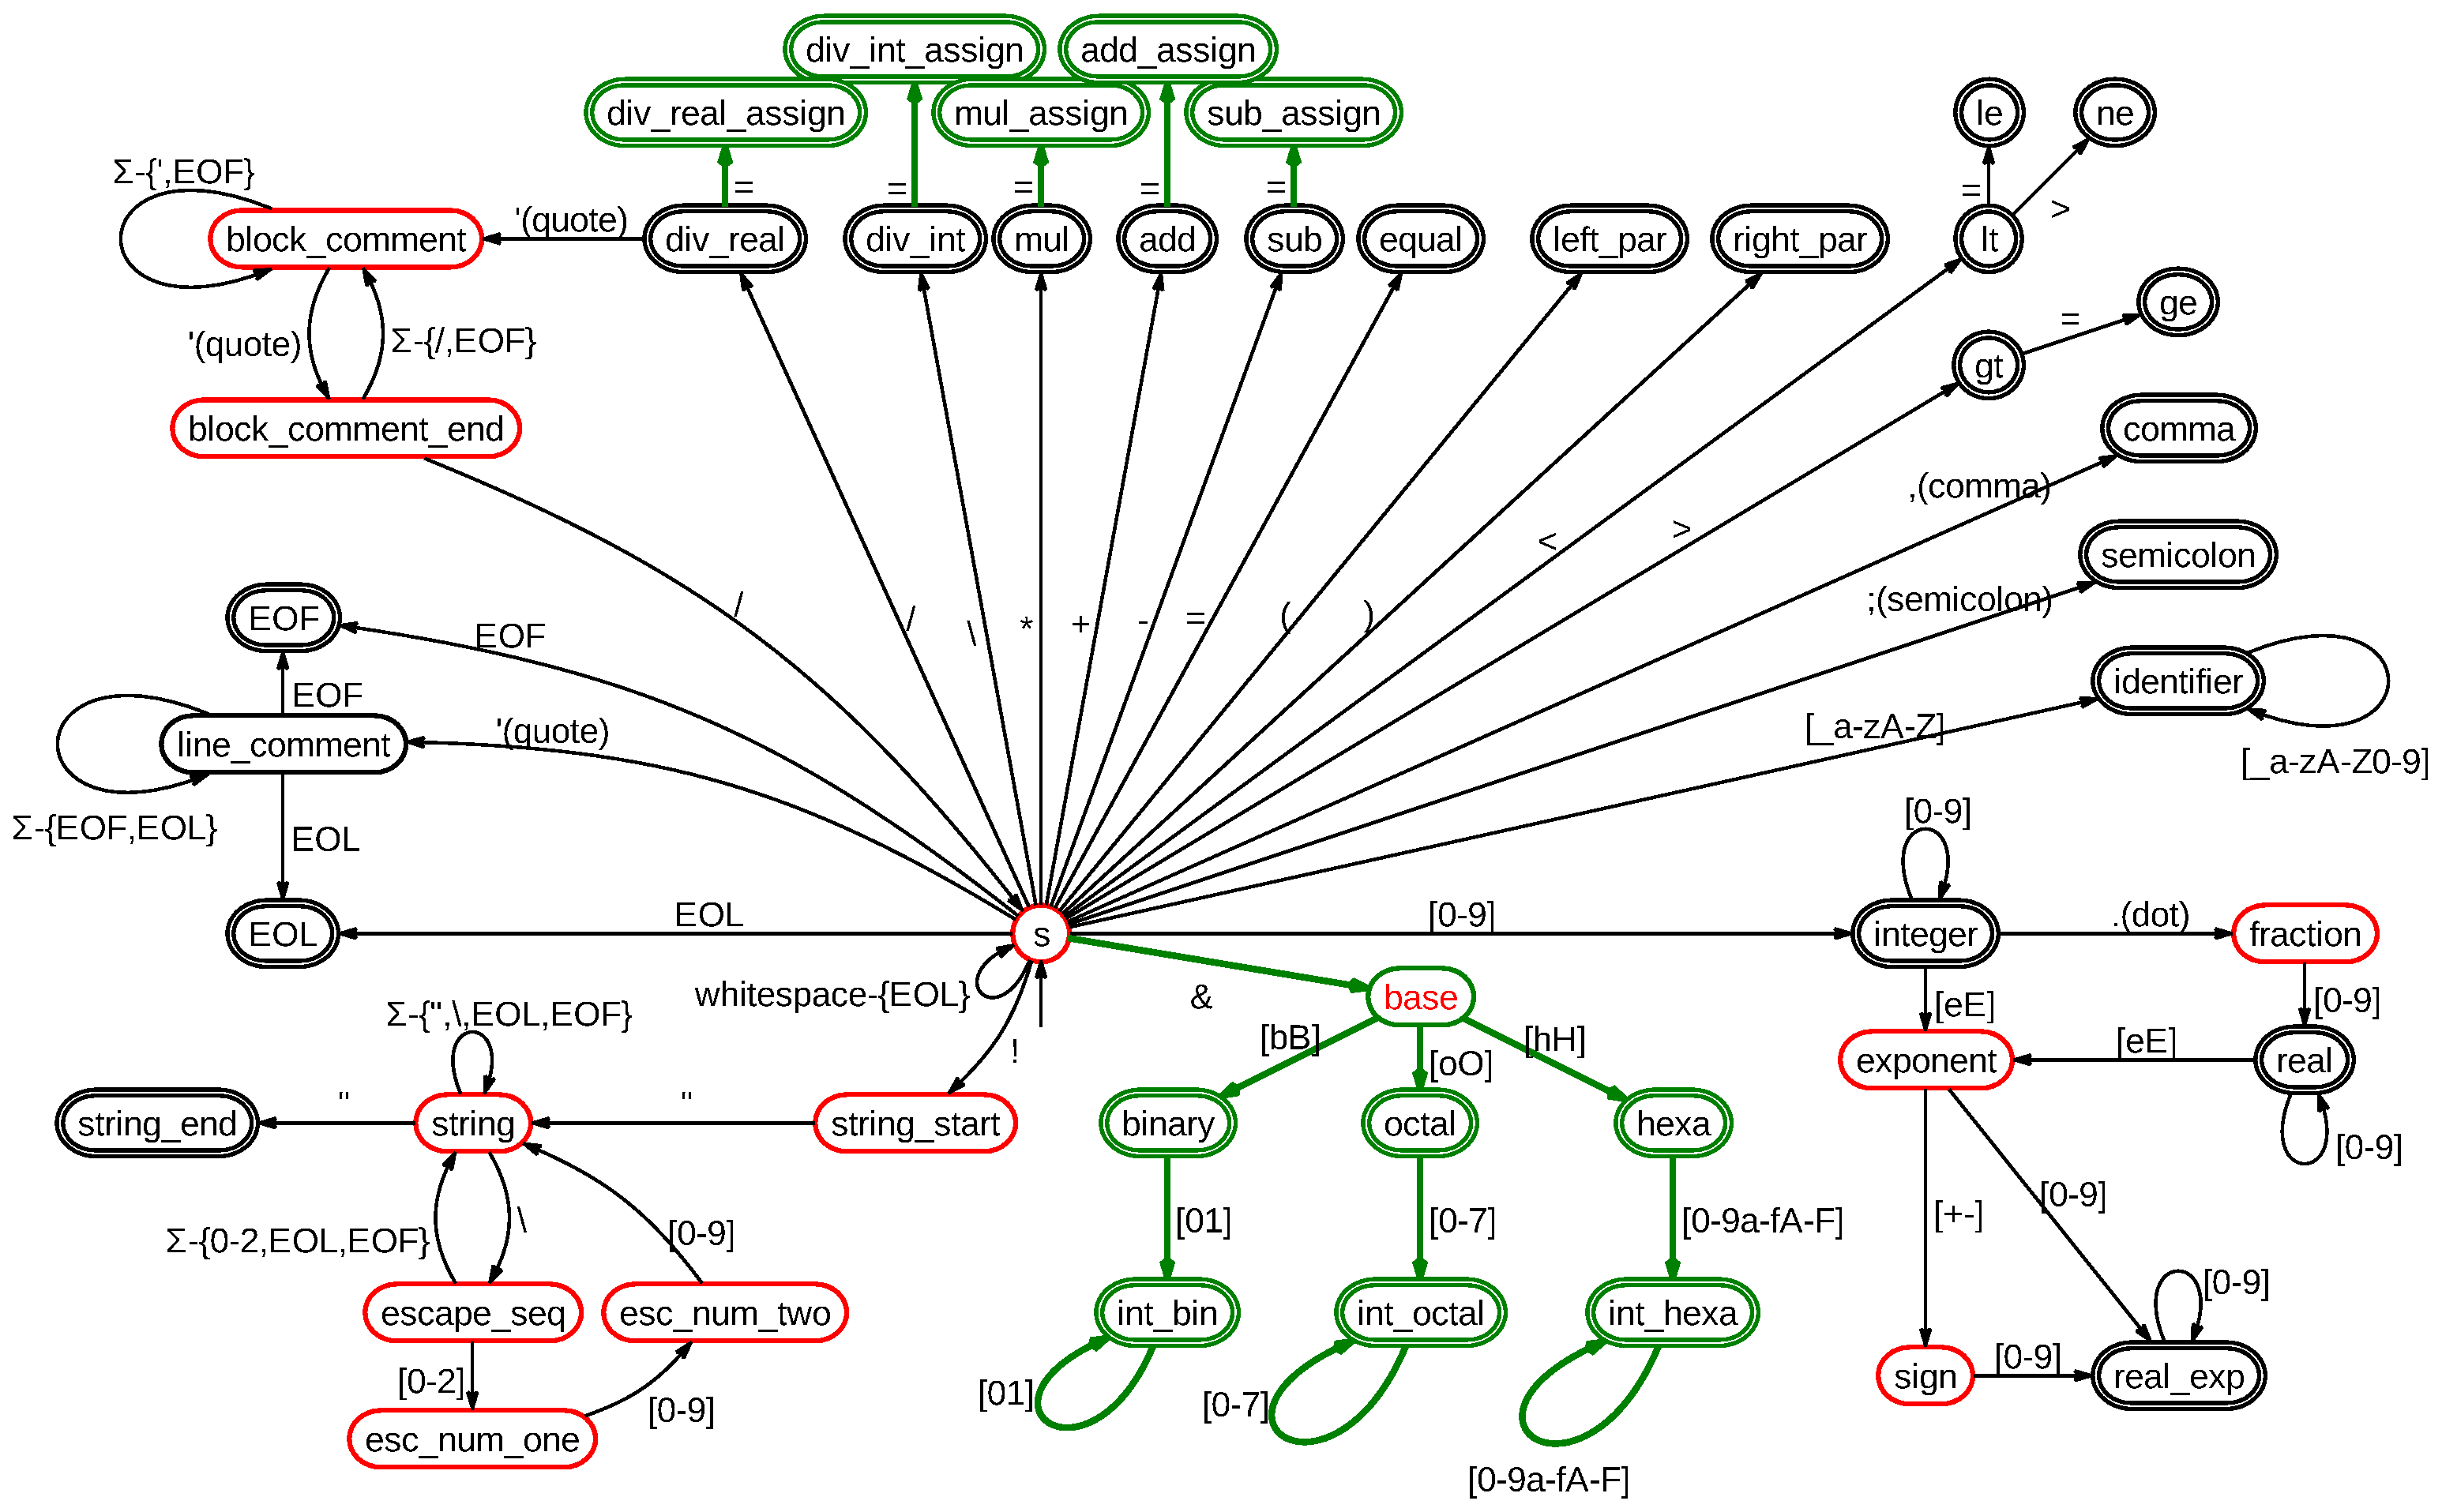
\includegraphics{images/scanner.eps}}
		\caption{Konečný automat specifikujicí lexikální analyzátor}
		\label{pic_scanner}
	\end{center}
\end{figure}
\clearpage
%-------------
% LL Gramatika
%-------------
\section*{LL Gramatika IFJ17}
\label{ll_grammar}
\small
\begin{eqnarray}
Line		&	\rightarrow		& GlobalStmt\quad ScopeStmt\quad  LineEnd	 \\
%###############################################################################
LineEnd		& \rightarrow		& \textbf{EOL}\quad LineEnd\\
			&		|			& \varepsilon		  \\
%###############################################################################
GlobalStmt	&	\rightarrow		&  FuncDecl\quad \textbf{EOL}\quad GlobalStmt	 \\
			&		|			& FuncDef\quad \textbf{EOL}\quad GlobalStmt    \\
			&		|			& \textcolor{green1}{SharedVar\quad \textbf{EOL}\quad GlobalStmt}	 \\
			&		|			& \textbf{EOL}\quad GlobalStmt\\
			&		|			& \varepsilon \\
%###############################################################################
InnerStmt	&	\rightarrow		& VarDecl  \\
			&		|			& Assignment	\\
			&		|			& IfStmt	\\
			&		|			& ScopeStmt   \\
			&		|			& DoStmt  \\
			&		|			& \textcolor{green1}{ForStmt}\quad	\\
			&		|			& PrintStmt \\
			&		|			& InputStmt  \\
			&		|			& ReturnStmt  \\
			&		|			& \textcolor{green1}{ExitStmt}	\\
			&		|			& \textcolor{green1}{ContinueStmt}	\\
			&		|			& \varepsilon \\
%###############################################################################
StmtSeq		&	 \rightarrow	& InnerStmt\quad \textbf{EOL}\quad StmtSeq	 \\
			&		|			& \varepsilon \\
%###############################################################################
VarDecl		& \rightarrow		& \textbf{DIM}\quad VarDef \\
			&		|			& \textcolor{green1}{\textbf{STATIC}\quad VarDef} \\
%###############################################################################
\textcolor{green1}{SharedVar}&		 \rightarrow		   & \textcolor{green1}{\textbf{DIM}\quad \textbf{SHARED}\quad VarDef} \\
%###############################################################################
VarDef		& \rightarrow		& \textbf{ID}\quad \textbf{AS}\quad Type \quad InitOpt\\
InitOpt		&	   \rightarrow	& `=`\quad Expression \\
			&		|			& \varepsilon \\
%###############################################################################
FuncDecl	&  \rightarrow		& \textbf{DECLARE}\quad \textbf{FUNCTION}\quad \textbf{ID}\quad `(` \quad Params \quad`)`\quad \textbf{AS}\quad Type   \\
%###############################################################################
Type		&	 \rightarrow	&	 \textbf{INTEGER}	 \\
			&		|			& \textbf{DOUBLE}	\\
			&		|			& \textbf{STRING}	\\
			&		|			& \textcolor{green1}{\textbf{BOOLEAN}}	\\
%###############################################################################
	FuncDef    &	\rightarrow    & \textbf{FUNCTION}\quad \textbf{ID}\quad `(`\quad Params\quad `)`\quad \textbf{AS}\quad Type\quad \textbf{EOL}\quad StmtSeq\quad \textbf{END}\quad \textbf{FUNCTION}\quad \\
%###############################################################################
ParamDecl	&	\rightarrow   & {\textbf{ID}\quad \textbf{AS}\quad Type}	\\
Params		&	 \rightarrow	& {ParamDecl}\quad ParamsNext  \\
			&	 |				& \varepsilon			  \\
ParamsNext	&	 \rightarrow	& `,`\quad {ParamDecl}\quad  ParamsNext   \\
			&	 |				& \varepsilon			  \\
%###############################################################################
ReturnStmt	&	\rightarrow		& \textbf{RETURN}\quad Expression	  \\
%###############################################################################
Assignment	& \rightarrow		& \textbf{ID}\quad AssignOperator \quad Expression \\
%###############################################################################
InputStmt	&	 \rightarrow	& \textbf{INPUT}\quad \textbf{ID}\quad	 \\
%###############################################################################
PrintStmt	&	 \rightarrow	& \textbf{PRINT}\quad Expression\quad `;` \quad ExpressionList\\
ExpressionList&  \rightarrow	&  Expression\quad `;`\quad ExpressionList\\
			&	 |				& \varepsilon	\\
%###############################################################################
ScopeStmt	&	 \rightarrow	&	\textbf{SCOPE}\quad   \textbf{EOL} \quad StmtSeq\quad	 \textbf{END}\quad \textbf{SCOPE}\quad	  \\
%###############################################################################
IfStmt	&\rightarrow& \textbf{IF} \quad Expression \quad \textbf{THEN}\quad \textbf{EOL}\quad StmtSeq \quad \textcolor{green1}{IfStmtElseif}\quad IfStmtElse\quad \textbf{END}\quad \textbf{IF}	\\
\textcolor{green1}{IfStmtElseif}&\rightarrow &\textcolor{green1}{\textbf{ELSEIF}\quad Expression\quad \textbf{THEN}\quad \textbf{EOL}\quad StmtSeq \quad IfStmtElseif}	 \\
&	|	&\textcolor{green1}{\varepsilon}  \\
IfStmtElse&   \rightarrow &\textbf{ELSE}\quad  \textbf{EOL}\quad StmtSeq\quad  \\
&	|	&\textcolor{green1}{\varepsilon}  \\
%###############################################################################
DoStmt&    \rightarrow	  & \textbf{DO} \quad DoStmtEnd   \\
DoStmtEnd&	 \rightarrow  &  TestTypeStart \quad  Expression \quad \textbf{EOL} \quad StmtSeq \quad \textbf{LOOP}	\\
&	 | &\textcolor{green1}{\textbf{EOL} \quad StmtSeq \quad \textbf{LOOP}\quad TestTypeEnd} \\
TestTypeStart & \rightarrow	&	\textbf{WHILE}\\
		&		|		& \textcolor{green1}{\textbf{UNTIL}} \\
\textcolor{green1}{TestTypeEnd} & \rightarrow	&	\textcolor{green1}{\textbf{WHILE}\quad Expression} \\
&		|		& \textcolor{green1}{\textbf{UNTIL}\quad Expression} \\
&	|	&\textcolor{green1}{\varepsilon}  \\
%###############################################################################
\textcolor{green1}{ExitStmt} & \rightarrow & \textcolor{green1}{\textbf{EXIT}\quad LoopType\quad LoopTypeEnd}	\\
%###############################################################################
\textcolor{green1}{ContinueStmt} & \rightarrow & \textcolor{green1}{\textbf{CONTINUE}\quad LoopType\quad LoopTypeEnd}	\\
%###############################################################################
\textcolor{green1}{LoopType} & \rightarrow & \textcolor{green1}{\textbf{DO}}\\
&	|		&	\textcolor{green1}{\textbf{FOR}}   \\
\textcolor{green1}{LoopTypeEnd} & \rightarrow & \textcolor{green1}{\textbf{,}\quad LoopType \quad LoopTypeEnd}\\
&	|		&	\textcolor{green1}{\varepsilon}   \\
%###############################################################################
\textcolor{green1}{ForStmt} &	 \rightarrow	&  \textcolor{green1}{\textbf{FOR}\quad \textbf{ID}\quad TypeOpt\quad `=`\quad Expression\quad \textbf{TO}\quad Expression\quad StepOpt\quad \textbf{EOL}\quad StmtSeq\quad \textbf{NEXT}\quad IdOpt\quad} \\
\textcolor{green1}{TypeOpt} & \rightarrow  & \textcolor{green1}{\textbf{AS}\quad Type} \\
& | &	\textcolor{green1}{\varepsilon} \\
\textcolor{green1}{StepOpt} & \rightarrow  & \textcolor{green1}{\textbf{STEP}\quad Expression} \\
& | &	\textcolor{green1}{\varepsilon} \\
\textcolor{green1}{IdOpt}	& \rightarrow & \textcolor{green1}{\textbf{ID}} \\
		& | &  \textcolor{green1}{\varepsilon} \\
%###############################################################################
AssignOperator	&	 \rightarrow	&	 `=` \quad		\\
		&	|		&	\textcolor{green1}{`-=`}	\\
		&	|		&	\textcolor{green1}{`+=`}	\\
		&	|		&	\textcolor{green1}{`*=`}	\\
		&	|		&	\textcolor{green1}{`\backslash =`} \\
		&	|		&	\textcolor{green1}{`/=`}	\\
%###############################################################################
%###############################################################################
\end{eqnarray}

\section*{Značení}
\begin{itemize}
\item{Neterminály: Vyznačeny kurzívou ($GlobalStmt$, $ScopeStmt$, \dots).}
\item{Terminály(tokeny): Zapsány velkými písmeny a vyznačeny tučně (\textbf{IF}, \textbf{LOOP}, \dots), případně ohraničeny v~apostrofech (`=`, `(`, `)`, \dots).}
\item[--]{Pravidla spjatá s~rozšířeními vyznačena \textcolor{green1}{zeleně}.}
\end{itemize}
%-------------------
% LL TABULKA
%-------------------
\begin{figure}[ht]
	\begin{center}
		\scalebox{0.5}{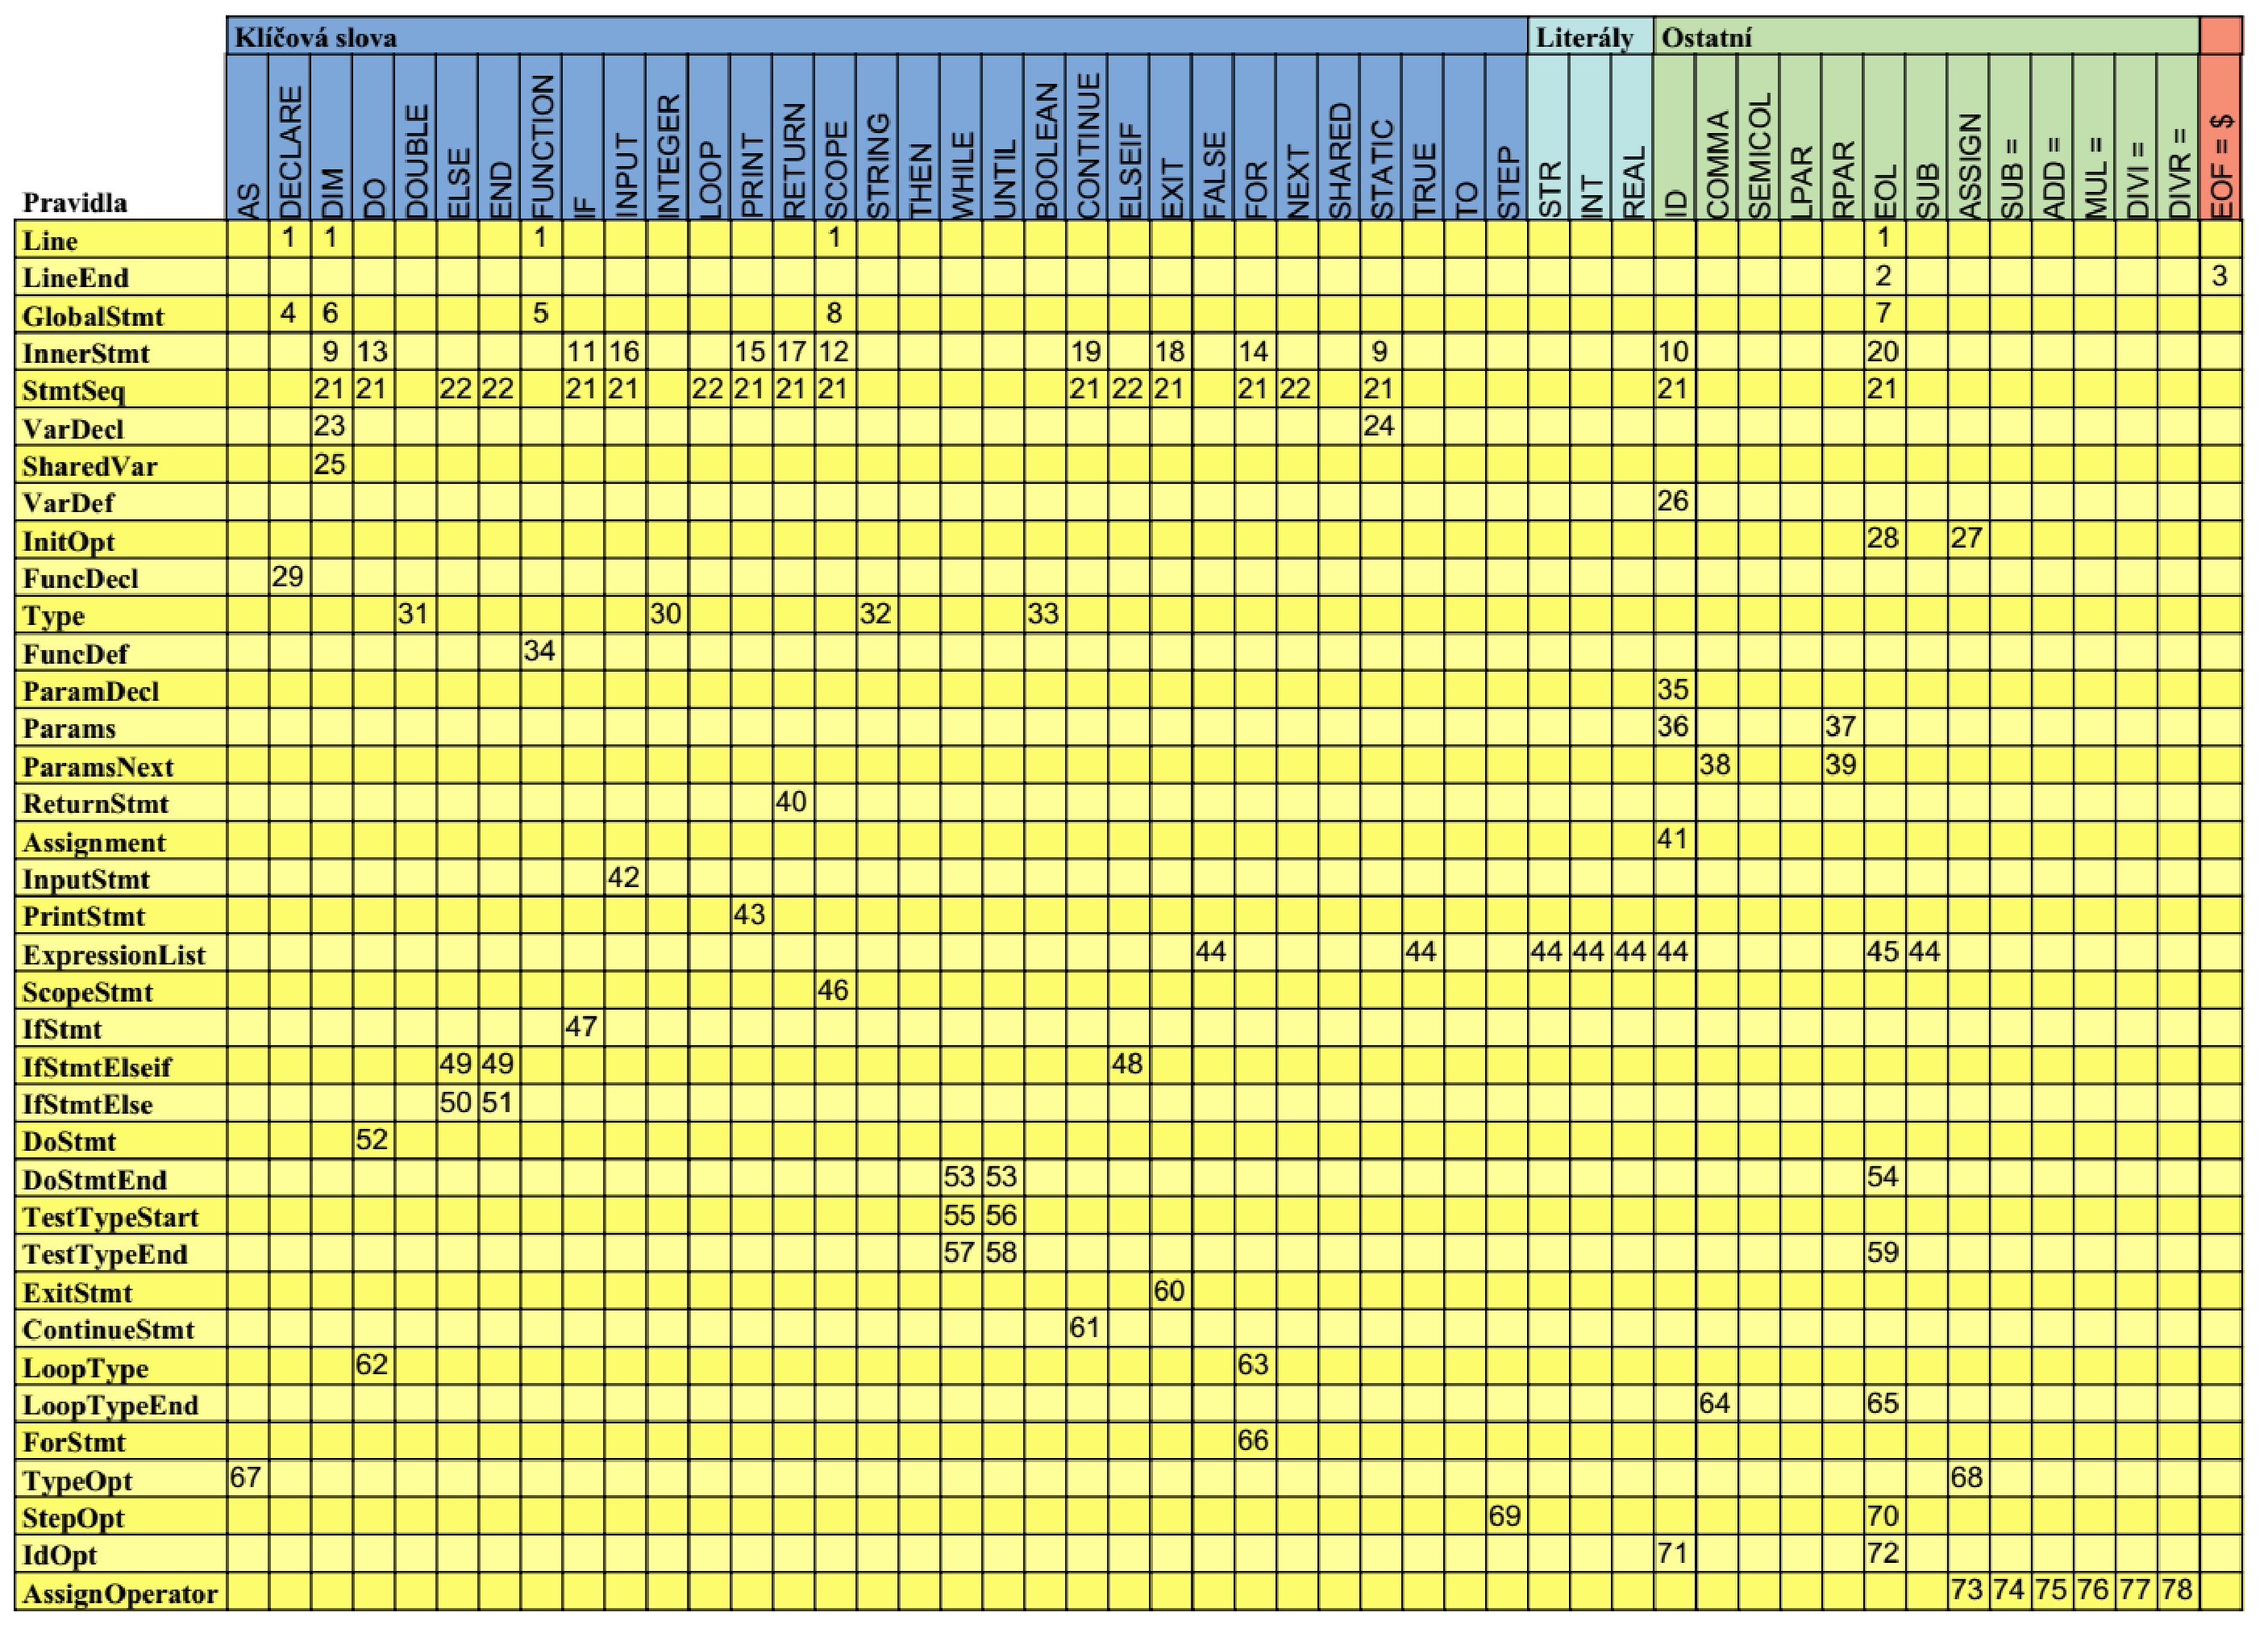
\includegraphics{images/ll-table.eps}}
		\caption{LL Tabulka}
		\label{pic_ll_table}
	\end{center}
\end{figure}
%-------------------
% PRECEDENCI TABULKA
%-------------------
\begin{figure}[ht]
	\begin{center}
		\scalebox{0.40}{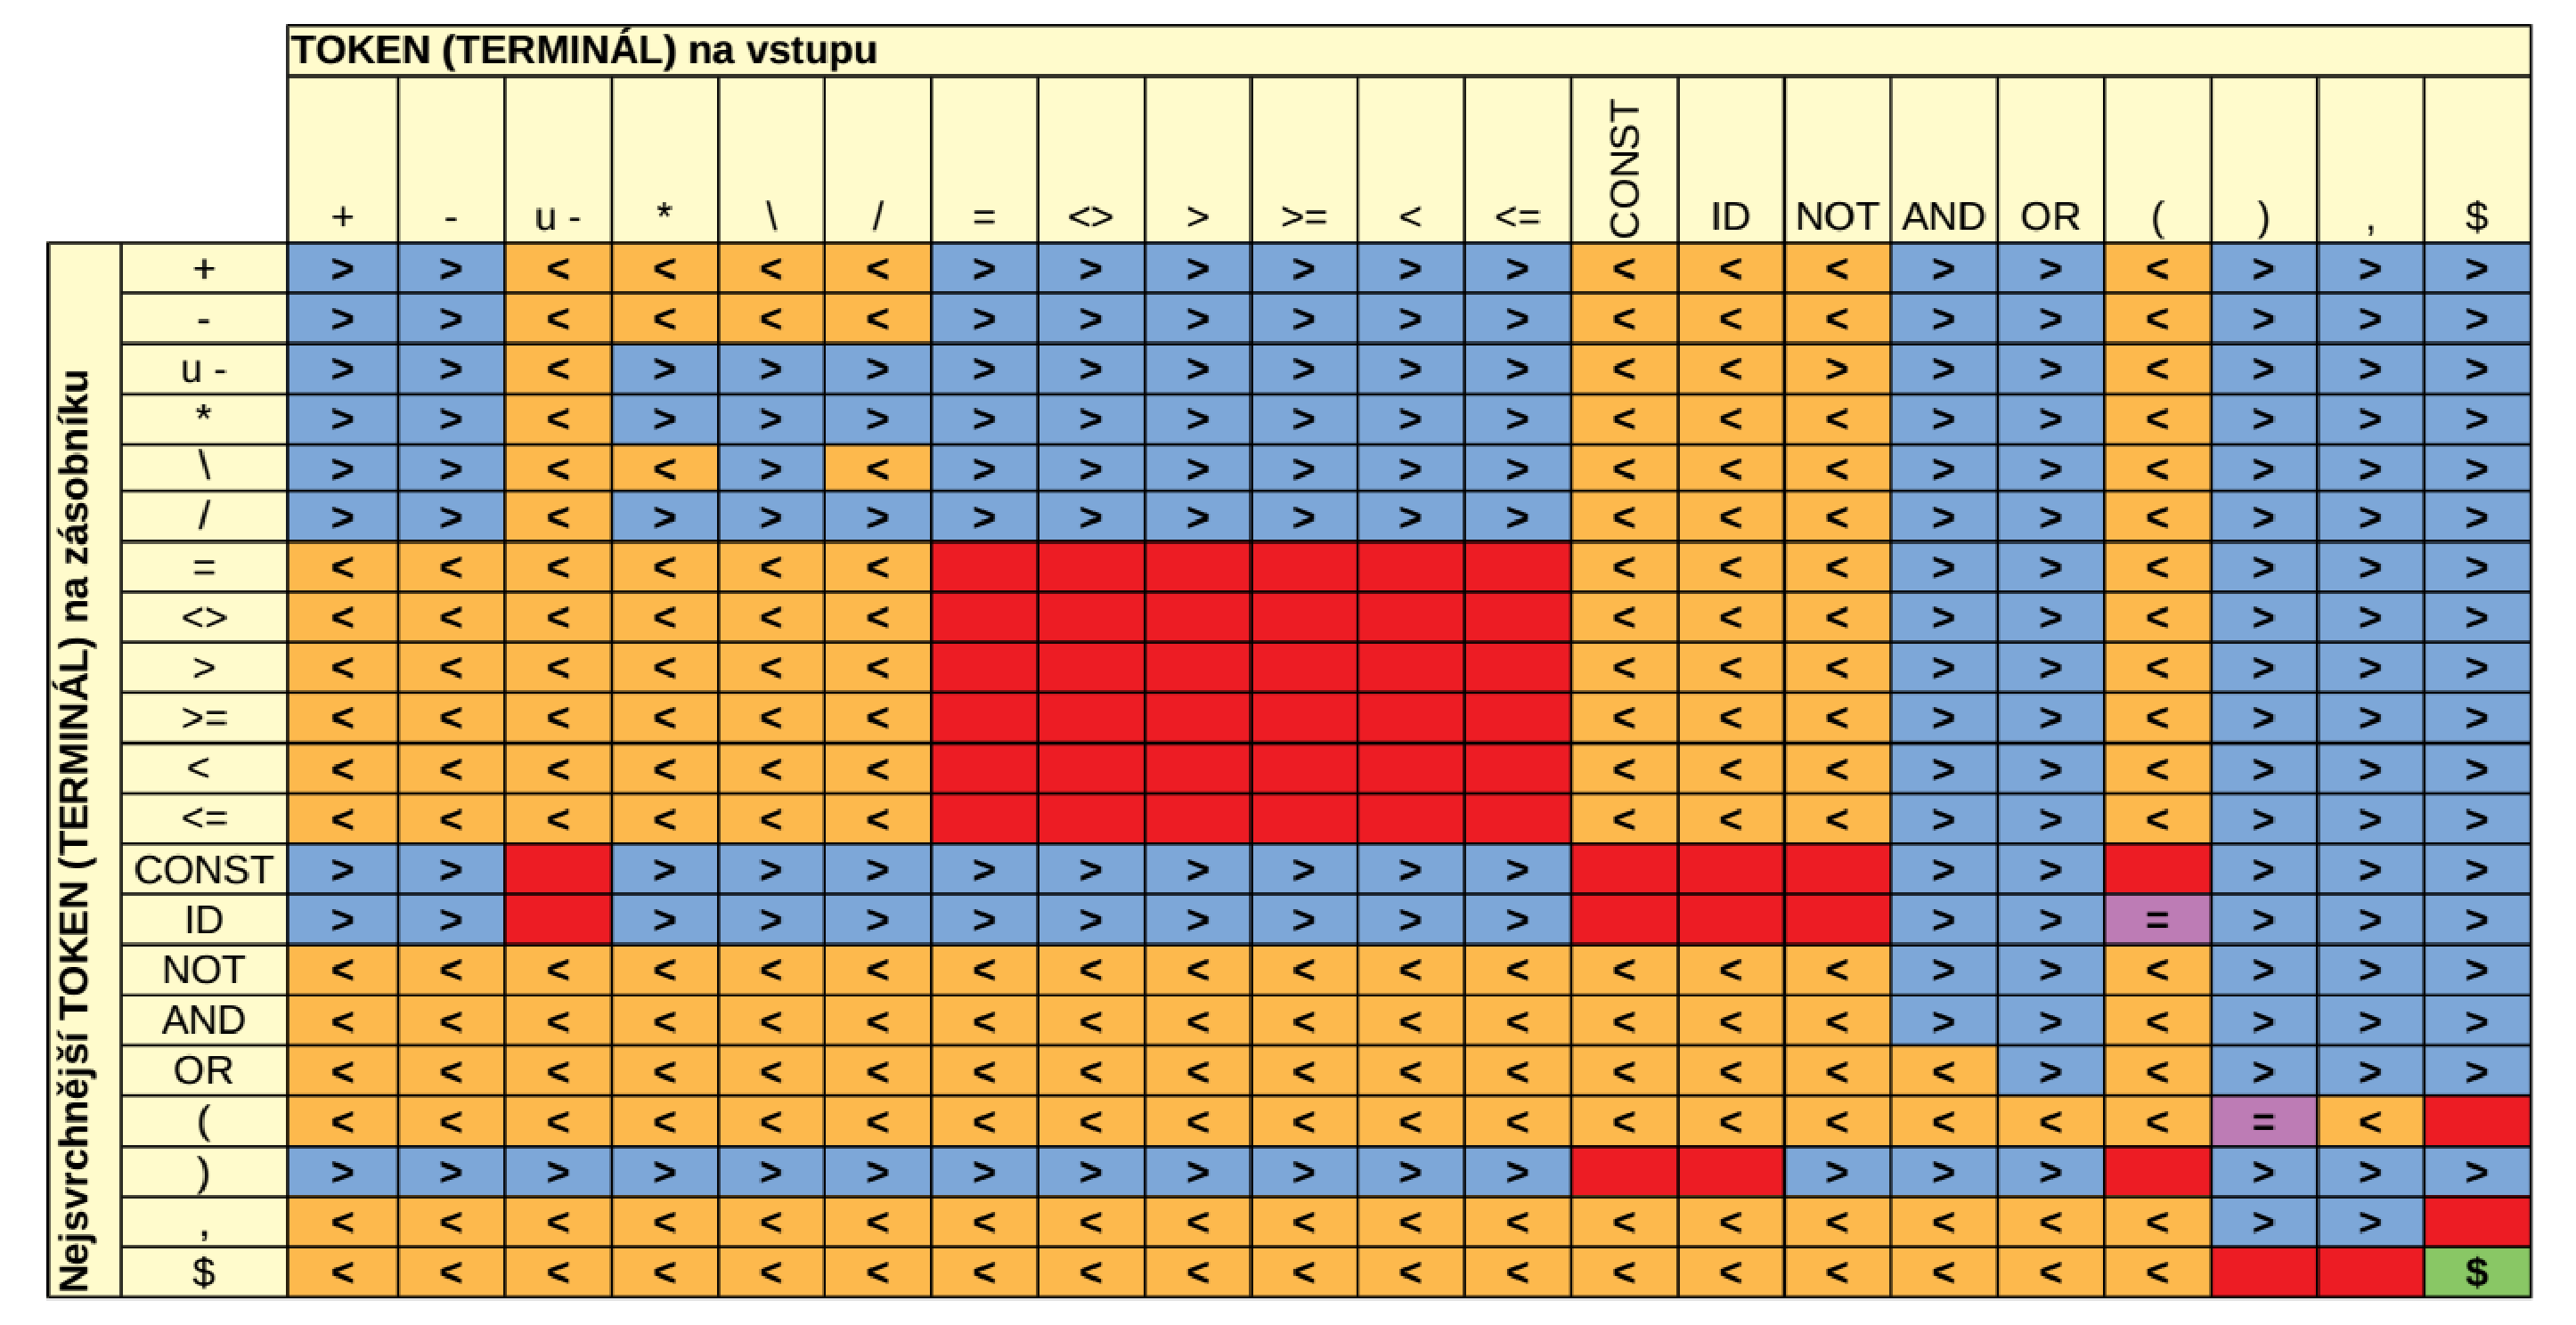
\includegraphics{images/prec-table.eps}}
		\caption{Precedenční tabulka}
		\label{pic_prec}
	\end{center}
\end{figure}
\end{landscape}
% %###############################################################################
\enddocument
